
\section{Session Establishment}
The session establishment uses different network methods to create connection to a peer. This also includes substitutions for situations where the default connection can not be established.

\subsection{Network Address Translation (NAT)}
Is used to give devices in a network a public IP address. This is achieved by translating requests from the device's private IP to the router's public IP with a unique port. The goal is to not need a unique public IP for each device.

\subsection{Session Traversal Utilities for NAT (STUN)}
This protocol is used to discover the public address of the peer. It also will determine any restrictions that would prevent a direct connection with a peer.

The peer sends a 'who am i' request to a STUN server which responds with the public address of the peer.

\begin{figure}[H]
	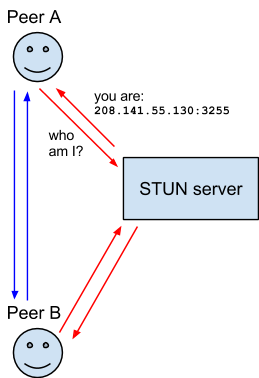
\includegraphics[scale=0.5]{images/webrtc-stun.png}
	\centering
	\caption{STUN communication schema, \url{https://developer.mozilla.org/en-US/docs/Web/API/WebRTC_API/Protocols}}
	\label{fig:STUN}
\end{figure}

There are open STUN servers available (list might not complete):
\begin{itemize}
	\item stun.l.google.com:19302
	\item stun[1-4].l.google.com:19302
	\item stunserver.org
	\item stun.schlund.de
	\item stun.voipstunt.com
\end{itemize}

\subsection{Traversal Using Relays around NAT (TURN)}
If STUN can't be used, because for example 'Symmetric NAT' is employed in the network, TURN will be used as fallback. This is achieved by opening a connection with a TURN server, this server then will relaying all information through that server.

\begin{figure}[H]
	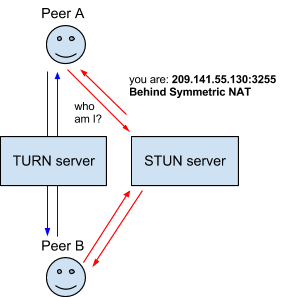
\includegraphics[scale=0.5]{images/webrtc-turn.png}
	\centering
	\caption{TURN communication schema, \url{https://developer.mozilla.org/en-US/docs/Web/API/WebRTC_API/Protocols}}
	\label{fig:TURN}
\end{figure}

There are open TURN servers, for example provided by google. But this will mean all communication is going threw a foreign server which might not be acceptable.

\subsection{Session Description Protocol (SDP)}
This standard describes the multimedia content of a connection. This includes a resolution, formats, codecs, encryption, etc. basically it is the metadata describing the content not the content itself.

\subsection{Interactive Connectivity Establishment (ICE) candidates}
Peers have to exchange information about the network connection, this is known as an ICE candidate. Each peer proposes its best candidate, and will work down to the worst candidate until they agree on a common candidate.

\subsection{Complete communication schema}
The following figure gives an overview over the complete communication mechanism. They also include the fallback mechanisms in case the default is not acceptable.

\begin{figure}[H]
	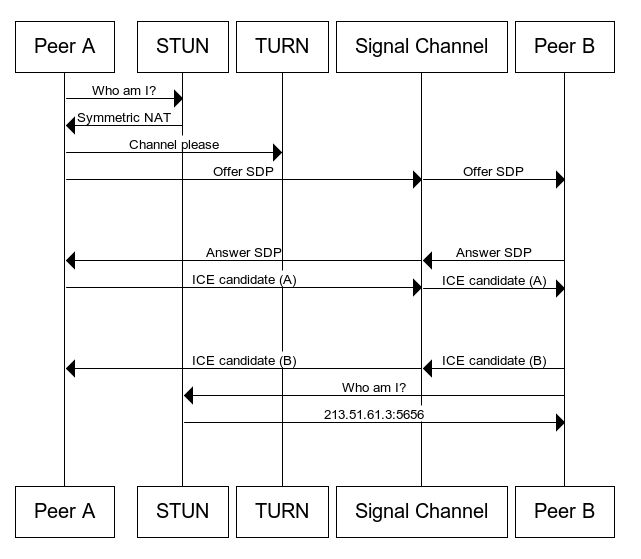
\includegraphics[scale=0.5]{images/webrtc-complete-diagram.png}
	\centering
	\caption{\Gls{webrtc} Complete communication schema, \url{https://developer.mozilla.org/en-US/docs/Web/API/WebRTC_API/Connectivity}}
	\label{fig:WebRTC}
\end{figure}

\section{Security}
Generally \Gls{webrtc} traffic is encrypted using Datagram Transport Layer Security (DTLS). Your data will be as secure as using any standard SSL based connection. Traffic that is relayed over a TURN server on the other hand is not necessarily end-to-end encrypted.

\textit{Confidentiality for the application data relayed by TURN is best provided by the application protocol itself, since running TURN over TLS does not protect application data between the server and the peer. If confidentiality of application data is important, then the application should encrypt or otherwise protect its data. For example, for real-time media, confidentiality can be provided by using SRTP.}~\cite{TURN:sec}
